\section{研究背景}
冗長自由度を有するヒトの身体を中枢神経系がどのように制御しているのかという問題は,ベルンシュタイン問題として知られており\cite{Bernstein1967},運動制御における古典的な未解決問題である.
この問題に対して,神経科学の分野では筋群の協調作用,すなわち,筋シナジーが冗長問題を解決する糸口になると期待されている.
筋シナジーは運動指令の機能的単位であり,制御自由度の数を減らす次元圧縮に貢献する.
そのため,多くの神経科学者が筋電位(EMG)から筋シナジーを抽出することで,ベルンシュタイン問題の解決を試みている\cite{Torres-Oviedo2007,Cappellini2006,d'Avella2005,Ivanenko2004,Ting2005,Ivanenko2006,Bizzi2008}.

Torres-Oviedoらは摂動を加えた時のヒトの姿勢制御中の16筋のEMGに多変量解析を適用することで,異なる摂動方向間で類似する筋シナジーを抽出した\cite{Torres-Oviedo2007}.
Cappelliniらはヒトの歩行や走行中の32筋のEMGに多変量解析を適用することで,タスク間で類似する4つの筋シナジーと各タスクで固有の1つの筋シナジーを抽出した\cite{Cappellini2006}.
d'Avellaらも多変量解析を用いて,カエルのジャンプ,水泳,歩行中の13筋のEMGからタスク間で類似する筋シナジーとタスク固有の筋シナジーを抽出した\cite{d'Avella2005}.
すなわち,運動学的,動力学的に大きく異なるタスク間で共通の筋シナジーが抽出された.
これらの結果は,我々が実行する運動タスクの種類に応じて理論上無数の筋シナジーが存在する可能性があるにも関わらず,少数の筋シナジーの重ね合わせで多彩な運動が実現されていることを示唆する.

しかし,先行研究の手法に共通する問題点として,平衡点と剛性という運動制御学的に重要な制御変数を考慮していないということが挙げられる.
ヒトの運動制御に関して古くから提唱されている平衡点仮説($\lambda$モデル)によれば,中枢神経系は身体の平衡点もしくは剛性を調整する2種類の運動指令を筋に送っている\cite{Feldman2008}.
そのため,EMGは平衡点と剛性の両方の情報を表現していると考えられ,EMGそのものに多変量解析を適用して筋シナジーを抽出しても,抽出される筋シナジーには両情報が混在してしまう.
その結果,筋シナジーが平衡点や剛性の制御に果たしている役割の評価が困難となる.

%また,先行研究の手法に共通するもう1つの問題点として,多変量解析を用いた筋シナジー抽出では,筋シナジーが平衡点や剛性の制御に及ぼす役割を定量評価できないということが挙げられる.
先行研究の手法に共通するもう1つの問題点として,多変量解析を用いた筋シナジー抽出では,筋シナジーの機能を定量的に評価できないということが挙げられる.
この問題を解決する1つの方法として,数理モデルを構築することが挙げられる.
なぜなら,筋シナジーと平衡点や剛性の関係を定式化できれば,筋シナジーが平衡点や剛性の制御に果たす役割を定量的に評価できるからである.

こうした中,我々はEMGを平衡点と剛性の情報に分離するために,筋拮抗比(A-A ratio)と筋拮抗和(A-A sum)という概念を提案し,筋骨格系の拮抗筋対の協調性を解析してきた\cite{Hirai2010,Iimura2011,Inoue2012,Ariga2013,Uno2014}.
ここで,筋拮抗比は拮抗筋対への運動コマンドの和に対する主導筋への運動コマンドの比として,筋拮抗和は拮抗筋対への運動コマンドの和として定義される.
そして,前者は平衡点の制御に,後者は剛性の制御に寄与することが,生体筋とよく似た特性を持つ人工筋のモデルにおいて理論的および実験的に実証されている\cite{Ariga2013}.
EMGをこれらの変量に変換することで,EMGから平衡点と剛性の情報を分離して抽出できることが期待される.
さらに近年,我々は筋拮抗比と筋拮抗和の概念を応用し,上肢/下肢運動に適用可能な数理モデルに基づく新しい筋シナジーの抽出法を提案している\cite{Uno2014}.
この数理モデルにおいて,身体の終点(エンドポイント)の平衡点は筋シナジーによって記述されるため,筋シナジーが平衡点の制御に果たす役割が明確になる.
我々はこの数理モデルに基づく筋シナジーの抽出法を上肢到達運動に適用することで,肩関節を中心とする極座標系において手先平衡点の動径,偏角方向の運動に寄与する2つの筋シナジーを抽出することに成功した\cite{Uno2014}.
さらに,数理モデルにおいて手先平衡点が筋シナジーによって記述されることを利用して,上肢運動中の手先平衡点軌道を推定することに成功している.

本研究では,筋シナジーが平衡点という運動学的な制御に果たす役割に着目した上で,数理モデルに基づく筋シナジーの抽出法を用いて,先行研究の2つの問題点を解決する.
そして,日常的に重要な下肢運動であるヒトの走行から平衡点の制御に果たす役割が明確な筋シナジーを抽出し,足先の平衡点軌道を推定する.
下肢運動中の足先平衡点軌道や足先剛性はその計測の難しさゆえに,実態はほとんど明らかにされていない.
そのため,足先の平衡点軌道や剛性の推定は大きな意義がある.
本研究では,筋拮抗比と筋拮抗和の概念を導入した上で,筋骨格モデルの力学解析に基づく筋協調解析を走行運動に適用し,筋シナジーの抽出,平衡点軌道と剛性の推定を行う.
そして,推定された平衡点軌道と剛性の妥当性をトルクやエネルギーの観点から考察する.
さらに,足先平衡点軌道をサブムーブメントの観点から考察し,サブムーブメントの抽出と抽出されたサブムーブメントの意味づけを行う.
本研究では以下のことを示す.
(1)抽出された筋シナジーは被験者に依らず,筋拮抗比の推移の大部分が動径方向と偏角方向の筋シナジーによって表現できる.
(2)筋協調解析により推定された平衡点軌道と剛性から算出した偏角方向のトルク,動径方向の力,足関節のトルクはそれぞれ,先行研究で逆動力学により算出された股関節,膝関節,足関節のモーメントと特徴が似ている.
(3)筋協調解析により推定された偏角方向と足関節の仕事率は重心の運動エネルギーと,偏角方向の仕事率は重心の位置エネルギーと密接に関係している.
 (4) 走行中の足先平衡点軌道は5つのサブムーブメントの重ね合わせによって表現でき,その数や発生タイミングは先行研究のものと類似している.
これらの結果は提案手法の妥当性を示すと同時に,ヒトが走行のようなリズミックな運動も離散的な運動コマンドによって生成していることを示唆するものである.

\section{力学解析に基づく筋協調解析}
本章では,ヒト下肢における筋骨格モデルの力学解析に基づく筋協調解析による筋シナジーの抽出法,足先平衡点軌道の推定法,足先剛性の推定法について述べる.

\subsection{筋骨格モデルの静力学}
%
\begin{figure}[!t]
 \begin{center}
  \includegraphics[width=0.5\columnwidth,clip]{eps/8muscles.eps}
  \caption{Musculoskeletal model of human lower limb. (A) Measurement muscles. (B) Simplified musculoskeletal model.}
  \label{8muscles}
 \end{center}
\end{figure}
%
ヒトの下肢のモデル({\bf Fig. \ref{8muscles}}(A))を模した{\bf Fig. \ref{8muscles}}(B)のような3対6筋の人工筋システムを考える\footnote{ここでは簡単のために足部を除いている.}.
このシステムは2つの関節とヒトの筋とよく似た特性を有する6つのマッキベン型の人工筋(PAM1~PAM6)とで構成されており,2つの関節は股関節と膝関節に対応し,6つの人工筋はヒトの6つの筋($m_1$~$m_6$)に対応している.
%このシステムはヒトの6つの筋($m_1$~$m_6$)に対応する6つの人工筋(PAM1~PAM6)と股関節と膝関節に対応する2つの関節で構成されている.
PAM$i$($i=1,\cdots,6$)の内部圧力を$P_i$,筋長を$l_i$,収縮力を$F_i$股関節と膝関節の角度を$\theta_{\rm h},\theta_{\rm k}$,平衡角度を$\theta_{\rm h,EP},\theta_{\rm k,EP}$,モーメントアームを$D$とする.
また,6つの人工筋の特性は同一のものとし,初期状態($\theta_{\rm h}=\theta_{{\rm h}0},\theta_{\rm k}=\theta_{{\rm k}0}$)における人工筋の内部圧力と筋長を$P_i=P_0$,$l_i=l_0$($i=1,\cdots,6$)とする.
我々はマッキベン型の人工筋は内部圧力$P_i$によって弾性係数$K(P_i)$と平衡長$l_{\rm EP}(P_i)$が変化するバネとして以下のように表現できることを力学解析と実験により実証している\cite{Ariga2013}.
\begin{eqnarray}
 \label{model1}
 F_i&=&K(P_i)(l_i-l_{\rm EP}(P_i))\\
 \label{model2}
 l_{\rm EP}(P_i)&=&\frac{C_1}{K(P_i)}+C_2\\
 \label{model3}
 K(P_i)&=&C_3(P_i-C_4)=C_3\cdot\hat{P}_i
\end{eqnarray}
%ただし,$F$は人工筋の収縮力,$l$は筋長であり.$C_1,C_2$は人工筋の自然長や損失係数などの特性から決まる定数である.
ただし,$C_1,C_2,C_3,C_4$は人工筋の自然長や損失係数などの特性から決まる定数であり,$\hat{P}_i=P_i-C_4$である.
また,$C_2$には$C_2<l_0$の関係がある.

ここでは,{\bf Fig. }\ref{8muscles}(B)の各関節に外力が働いておらず,かつ静的な状態を考える.
このとき,関節角度と関節平衡角度が等しいので,
\begin{eqnarray}
 \label{Eangle1}
 \theta_{\rm h}&=&\theta_{\rm h,EP},\\
 \label{Eangle2}
 \theta_{\rm k}&=&\theta_{\rm k,EP},
\end{eqnarray}
が成り立つ.また,力のつり合いより,
\begin{eqnarray}
 \label{balance1}
 F_1-F_2+F_3-F_4&=&0,\\
 \label{balance2}
 -F_3+F_4+F_5-F_6&=&0,
\end{eqnarray}
が成り立つ.
%ので,Eq. (\ref{PAMmodel})より,
%\begin{eqnarray}
% K(P_1){l_1-l_0(P_1)}-K(P_2){l_2-l_0(P_2)}\nonumber \\
% +K(P_3){l_3-l_0(P_3)}-K(P_4){l_4-l_0(P_4)}=0,\\
% -K(P_3){l_3-l_0(P_3)}+K(P_4){l_4-l_0(P_4)}\nonumber \\
% +K(P_5){l_5-l_0(P_5)}-K(P_6){l_6-l_0(P_6)}=0,
%\end{eqnarray}
%が成り立つ.
さらに,関節角度の初期状態からの変位を$\Delta\theta_{\rm h}=\theta_{\rm h}-\theta_{{\rm h}0},\Delta\theta_{\rm k}=\theta_{\rm k}-\theta_{{\rm k}0}$とすると,幾何関係より,
\begin{eqnarray}
 \label{geo1}
 D\cdot\Delta\theta_{\rm h}&=l_1-l_0=&-(l_2-l_0),\\
 \label{geo2}
 D(\Delta\theta_{\rm h}-\Delta\theta_{\rm k})&=l_3-l_0=&-(l_4-l_0),\\
 \label{geo3}
 D\cdot\Delta\theta_{\rm k}&=l_5-l_0=&-(l_6-l_0),
\end{eqnarray}
が成り立つ.
そして,Eqs. (\ref{balance1}),(\ref{balance2})にEq. (\ref{model1})を代入し,Eqs. (\ref{model2}),(\ref{model3}),(\ref{geo1}),(\ref{geo2}),(\ref{geo3})を用いて整理すると関節角度と人工筋の圧力との関係に関する以下の式を得る.
\begin{eqnarray*}
 \arraycolsep=1.5pt
 \label{mat1}
 \left[
  \begin{array}{cc}
   \hat{P}_1+\hat{P}_2+\hat{P}_3+\hat{P}_4 & -(\hat{P}_3+\hat{P}_4) \\
   -(\hat{P}_3+\hat{P}_4) & \hat{P}_3+\hat{P}_4+\hat{P}_5+\hat{P}_6
  \end{array}
 \right]
 \left[
  \begin{array}{c}
   \Delta\theta_{\rm h} \\
   \Delta\theta_{\rm k}
  \end{array}
 \right]
\end{eqnarray*}
\vspace{-1.em}
\begin{eqnarray}
 \arraycolsep=1.5pt
 \label{mat2}
 =\frac{l_0-C_2}{D}
 \left[
  \begin{array}{c}
   \hat{P}_1-\hat{P}_2+\hat{P}_3-\hat{P}_4 \\
   -(\hat{P}_3-\hat{P}_4-\hat{P}_5+\hat{P}_6)
  \end{array}
 \right]
\end{eqnarray}

\subsection{筋拮抗比・筋拮抗和の導入とシナジーベクトル}
さらに,筋拮抗比$r_i$[-]と筋拮抗和$s_i$[Pa],($i=1,2,3$)を以下のように定義する\cite{Ariga2013}.
\begin{eqnarray}
 \label{def_sum}
 r_i&=&\frac{\hat{P}_{2i-1}}{\hat{P}_{2i-1}+\hat{P}_{2i}} \\
 \label{def_ratio}
 s_i&=&\hat{P}_{2i-1}+\hat{P}_{2i}
\end{eqnarray}
%
\begin{table}[t]
 \caption{Definition of the A-A ratio and the A-A sum for artificial muscle system.}
 \begin{center}
  \scalebox{1}{
   \begin{tabular}{|c|c|c|} \hline
    Label & Definition & Motor function \\ \hline \hline
    $r_1$ & $P_1/(P_1+P_2)$ & Hip extention \\
    $r_2$ & $P_3/(P_3+P_4)$ & Hip extention and knee flexion \\
    $r_3$ & $P_5/(P_5+P_6)$ & Knee extention \\ \hline
    $s_1$ & $P_1+P_2$ & Hip-joint stiffness increase\\
    $s_2$ & $P_3+P_4$ & Hip and knee-joint stiffness increase\\
    $s_3$ & $P_5+P_6$ & Knee-joint stiffness increase\\ \hline
   \end{tabular}
   \label{def_rs}
  }
 \end{center}
\end{table}
%
それぞれの筋拮抗比と筋拮抗和の機能を{\bf Table} \ref{def_rs}に示す.
$r_i,s_i,(i=1,2,3$)を用いてEq. (\ref{mat2})を変形すると以下のようになる.
\begin{eqnarray}
 \arraycolsep=1.5pt
 \label{mat3}
 \left[
  \begin{array}{c}
   \Delta\theta_{\rm h} \\
   \Delta\theta_{\rm k}
  \end{array}
 \right]=\frac{2(l_0-C_2)}{D}
 \left[
  \begin{array}{c}
   \ve{q}^{\rm T}_1 \\
   \ve{q}^{\rm T}_2
  \end{array}
 \right]
 \left[
  \begin{array}{c}
   r_{1}-\frac{1}{2} \\
   r_{2}-\frac{1}{2} \\
   r_{3}-\frac{1}{2} \\
  \end{array}
 \right]
\end{eqnarray}
ただし,
\begin{eqnarray}
 \arraycolsep=1.5pt
 \ve{q}_1=\frac{1}{s_{1}s_{2}+s_{2}s_{3}+s_{3}s_{1}}
 \left[
  \begin{array}{c}
   -s_{1}s_{2}-s_{3}s_{1} \\
   -s_{2}s_{3} \\
   -s_{2}s_{3}
  \end{array}
 \right],
 \label{q1}
\end{eqnarray}
\begin{eqnarray}
 \arraycolsep=1.5pt
 \ve{q}_2=\frac{1}{s_{1}s_{2}+s_{2}s_{3}+s_{3}s_{1}}
 \left[
  \begin{array}{c}
   -s_{1}s_{2} \\
   s_{1}s_{2} \\
   -s_{2}s_{3}-s_{3}s_{1}
  \end{array}
 \right],
 \label{q2}
\end{eqnarray}
である.
これは,$\ve{q}_1,\ve{q}_2$が一定であれば,関節変位と筋拮抗比に線形関係が成り立つことを意味する.
さらに,関節平衡角度$(\theta_{\rm h,EP},\theta_{\rm k,EP})$と極座標における足先平衡位置$(R_{\rm EP},{\it \Phi}_{\rm EP})$には以下の線形に近い関係がある\cite{Mitsuda1996}.
\begin{eqnarray}
 \arraycolsep=1.5pt
 \left[
  \begin{array}{c}
   \dot{R}_{\rm EP} \\
   \dot{\it \Phi}_{\rm EP}
  \end{array}
 \right]
 =
 \left[
  \begin{array}{cc}
   0 & -L{\rm sin}(\theta_{\rm k,EP}/2) \\ %-L{\rm sin}\frac{\theta_{\rm k,EP}}{2} \\
   1 & -\frac{1}{2}
  \end{array}
 \right]
 \left[
  \begin{array}{c}
   \dot{\theta}_{\rm h,EP} \\
   \dot{\theta}_{\rm k,EP}
  \end{array}
 \right]
 \label{jacobi}
\end{eqnarray}
%時間微分するには平衡角度にしておく必要がある.なぜなら,ダイナミクスの影響により,筋拮抗比の変化と足先位置の変化は一致しないからである.
そして,$\ve{q}_1,\ve{q}_2$が平衡点周りで一定であるという仮定の下,Eq. (\ref{mat3})にEqs (\ref{Eangle1},\ref{Eangle2})を代入した上で両辺を$t$で微分し,その結果をEq. (\ref{jacobi})に代入すると以下の式を得る.
\begin{eqnarray}
 \label{def_synergy}
 \arraycolsep=0.3pt
 \left[
  \begin{array}{c}
   \dot{R}_{\rm EP} \\
   \dot{\it \Phi}_{\rm EP}
  \end{array}
 \right]
 =
 \left[
  \begin{array}{cc}
   C_5(\theta_{\rm k,EP}) & 0 \\
   0 & C_6
  \end{array}
 \right]
 \left[
  \begin{array}{c}
   \ve{q}_2^{\rm T} \\
   (\ve{q}_1-\frac{1}{2}\ve{q}_2)^{\rm T}
  \end{array}
 \right]
 \left[
  \begin{array}{c}
   \dot{r}_{1} \\
   \dot{r}_{2} \\
   \dot{r}_{3}
  \end{array}
 \right]
\end{eqnarray}
ここで,$C_5(\theta_{\rm k,EP})=-\frac{2L(l_0-C_2)}{D}{\rm sin}(\theta_{\rm k,EP}/2)(<0),C_6=\frac{2(l_0-C_2)}{D}(>0)$は人工筋の特性,リンク長,モーメントアーム,膝関節の平衡角度$\theta_{\rm k,EP}$によって決まる値である.
Eq. (\ref{def_synergy})は筋拮抗比の速度のベクトル$\dot{\ve{r}}(t)=(\dot{r}_{1}(t),\dot{r}_{2}(t),\dot{r}_{3}(t))^{\rm T}$を筋拮抗和に依存して決まる2つのベクトル$\ve{q}_2$および$\ve{q}_1-\frac{1}{2}\ve{q}_2$によって張られる部分空間へ射影することで,足先の平衡点の速度を推定できることを示している.
%したがって,$\ve{s}_2$は動径方向,$\ve{s}_1-\frac{1}{2}\ve{s}_2$は偏角方向の運動に寄与するベクトルといえる.
また,$\ve{q}_2$と$\ve{q}_1-\frac{1}{2}\ve{q}_2$に直交するベクトルは足先の平衡点の変化に直接寄与しない.
動径方向,偏角方向,動径と偏角に直交する方向の基底ベクトルを求めると,
\begin{eqnarray}
 \ve{u}_R=\ve{q}_2/|\ve{q}_2|,\\
 \ve{u}_{\it \Phi}=(\ve{q}_1-\frac{1}{2}\ve{q}_2)/|\ve{q}_1-\frac{1}{2}\ve{q}_2|,\\
 \ve{u}_{R\times{\it \Phi}}=(\ve{q}_R\times\ve{q}_{\it \Phi})/|(\ve{q}_R\times\ve{q}_{\it \Phi})|,
\end{eqnarray}
となる.
以下,$\ve{u}_R,\ve{u}_{\it \Phi},\ve{u}_{R\times{\it \Phi}}$をそれぞれ動径方向,偏角方向,零空間のシナジーベクトルと定義する.
%そして,シナジーベクトルと筋拮抗比の変化量$d\ve{r}=\ve{r}-\bar{\ve{r}}$との内積をシナジースコアと定義する.
シナジーベクトル$\ve{u}_R,\ve{u}_{\it \Phi},\ve{u}_{R\times{\it \Phi}}$は筋群の協調を重み付きでベクトル化したものである.
以下,シナジーベクトル$\ve{u}_R,\ve{u}_{\it \Phi},\ve{u}_{R\times{\it \Phi}}$を力学解析に基づき抽出された筋シナジーとする.
そして,シナジーベクトルは筋拮抗和によってのみ表現されるので,シナジーベクトルは関節剛性に寄与する指令値によって定まると考えることができる.

\subsection{足先平衡点軌道の推定}
本節では,筋骨格モデルの力学解析に基づく足先平衡点軌道の推定方法について述べる.
シナジーベクトルと筋拮抗比$r_i(t)\;(i=1,\cdots,3)$の時間標本平均からの変化量$d\ve{r}(t)=\ve{r}(t)-\bar{\ve{r}}$との内積$w_R=\ve{u}_R.d\ve{r},w_{\it \Phi}=\ve{u}_{\it \Phi}.d\ve{r},w_{R\times{\it \Phi}}=\ve{u}_{R\times{\it \Phi}}.d\ve{r}$を動径,偏角,零空間のシナジースコアと定義する.
Eq. (\ref{def_synergy})に,$\ve{u}_R,\ve{u}_{\it \Phi}$を代入し,時間で積分すると以下の関係が得られる.
\begin{eqnarray}
 -R\propto\ve{u}_R.d\ve{r}=w_R\\
 {\it \Phi}\propto\ve{u}_{\it \Phi}.d\ve{r}=w_{\it \Phi}
\end{eqnarray}
したがって,シナジースコア$w_R,w_{\it \Phi}$を適切に線形変換することで,極座標における足先の動径方向と偏角方向の平衡点軌道$(R_{\rm EP},{\it \Phi}_{\rm EP})$を推定できる.
シナジースコアの線形変換には以下の式を用いる.
\begin{eqnarray}
 R_{\rm EP}=\frac{R_{\rm max}-R_{\rm min}}{w^*_{R,{\rm max}}-w^*_{R,{\rm min}}}(w^*_R-w^*_{R,{\rm min}})+R_{\rm min}\\
 {\it \Phi}_{\rm EP}=\frac{{\it \Phi}_{\rm max}-{\it \Phi}_{\rm min}}{w_{{\it \Phi},{\rm max}}-w_{{\it \Phi},{\rm min}}}(w_{\it \Phi}-w_{{\it \Phi},{\rm min}})+{\it \Phi}_{\rm min}
\end{eqnarray}
ここで,$R_{\rm max},R_{\rm min},{\it \Phi}_{\rm max},{\it \Phi}_{\rm min}$はそれぞれタスク中の$R$と${\it \Phi}$の最大値と最小値であり,$w^*_{R,{\rm max}},$
$w^*_{R,{\rm min}},w_{{\it \Phi},{\rm max}},w_{{\it \Phi},{\rm min}}$はそれぞれタスク中の$w^*_R=-w_R$と$w_{\it \Phi}$の最大値と最小値である.
%$(R_{\rm EP},{\it \Phi}_{\rm EP})$を$x-y$空間に変換した$(x_{\rm EP},y_{\rm EP})=(R_{\rm EP}{\rm cos}({\it \Phi}_{\rm EP}),-R_{\rm EP}{\rm sin}({\it \Phi}_{\rm EP}))$をEMGから推定した足先平衡点軌道とする.
$(R_{\rm EP},{\it \Phi}_{\rm EP})$を筋活動から推定した足先平衡点軌道とする.

\subsection{足先剛性の推定}
%
\begin{figure}[!t]
 \begin{center}
  \includegraphics[width=0.3\columnwidth,clip]{eps/def_stiffness.eps}
  \caption{Definition of stiffness in radial direction $K_R$ and that in angular direction $K_{\it \Phi}$}
  \label{def_stiffness2}
 \end{center}
\end{figure}
%
本節では,筋骨格モデルの力学解析に基づく足先剛性の推定方法について述べる.
{\bf Fig. }\ref{8muscles}(B)の平衡状態から足先に外力を加えたとき,股関節と膝関節にそれぞれ$\tau_{\rm h},\tau_{\rm k}$のトルク(トルクの正方向は関節角の正方向と同じとする)が作用し,平衡状態から股関節と膝関節がそれぞれ$\Delta\theta'_{\rm h},\Delta\theta'_{\rm k}$変化して,$\theta_{\rm h}=\Delta\theta_{\rm h}+\Delta\theta'_{\rm h},\theta_{\rm k}=\Delta\theta_{\rm k}+\Delta\theta'_{\rm k}$で外力とつり合ったとする.
そして,このときのPAM$i$($i=1,\cdots,6$)の筋長を$l'_i$,収縮力を$F'_i$とすると,力のつり合いより,
\begin{eqnarray}
 \label{balance3}
 \tau_{\rm h}=D(F'_1-F'_2+F'_3-F'_4),\\
 \label{balance4}
 \tau_{\rm k}=D(-F'_3+F'_4+F'_5-F'_6),
\end{eqnarray}
が成り立つ.
%ので,Eq. (\ref{PAMmodel})より,
%\begin{eqnarray}
% K(P_1){l_1-l_0(P_1)}-K(P_2){l_2-l_0(P_2)}\nonumber \\
% +K(P_3){l_3-l_0(P_3)}-K(P_4){l_4-l_0(P_4)}=0,\\
% -K(P_3){l_3-l_0(P_3)}+K(P_4){l_4-l_0(P_4)}\nonumber \\
% +K(P_5){l_5-l_0(P_5)}-K(P_6){l_6-l_0(P_6)}=0,
%\end{eqnarray}
%が成り立つ.
また,幾何関係より,
\begin{eqnarray}
 \label{geo4}
 D(\Delta\theta_{\rm h}+\Delta\theta'_{\rm h})=l'_1-l_0=-(l'_2-l_0),\\
 \label{geo5}
 D\{(\Delta\theta_{\rm h}+\Delta\theta'_{\rm h})-(\Delta\theta_{\rm k}+\Delta\theta'_{\rm k})\}=l'_3-l_0=-(l'_4-l_0),\\
 \label{geo6}
 D(\Delta\theta_{\rm k}+\Delta\theta'_{\rm k})=l'_5-l_0=-(l'_6-l_0),
\end{eqnarray}
が成り立つ.
したがって,Eqs. (\ref{balance3},\ref{balance4})にEqs. (\ref{model1},\ref{model2})を代入し,Eqs. (\ref{model3},\ref{geo4},\ref{geo5},\ref{geo6})を用いて整理すると以下の式を得る.
\begin{eqnarray}
 \label{mat4}
 \left[
  \begin{array}{c}
   \tau_{\rm h} \\
   \tau_{\rm k}
  \end{array}
 \right]
 \hspace{-0.5em}&=&\hspace{-0.5em}D^2
 \left[
  \begin{array}{c}
   (K(P_1)+K(P_2))\Delta\theta'_{\rm h}+(K(P_3)+K(P_4))(\Delta\theta'_{\rm h}-\Delta\theta'_{\rm k}) \\
   -(K(P_3)+K(P_4))(\Delta\theta'_{\rm h}-\Delta\theta'_{\rm k})+(K(P_5)+K(P_6))\Delta\theta'_{\rm k}
  \end{array}
 \right] \nonumber \\
 &=&\hspace{-0.5em}C_3D^2
 \left[
  \begin{array}{cc}
   s_1+s_2 & -s_2 \\
   -s_2 & s_2+s_3
  \end{array}
 \right]
 \left[
  \begin{array}{c}
   \theta'_{\rm h} \\
   \theta'_{\rm k}
  \end{array}
 \right]
\end{eqnarray}
Eq. (\ref{mat4})より,関節剛性$\ve{K}_{\theta}=\frac{\partial(\tau_{\rm h},\tau_{\rm k})^{\rm T}}{\partial(\theta_{\rm h},\theta_{\rm k})}$は以下のようになる.
\begin{eqnarray}
 \label{joint_stiffness}
 \ve{K}_{\theta}=C_3D^2
 \left[
  \begin{array}{cc}
   s_1+s_2 & -s_2 \\
   -s_2 & s_2+s_3
  \end{array}
 \right]=C_7
 \left[
  \begin{array}{cc}
   s_1+s_2 & -s_2 \\
   -s_2 & s_2+s_3
  \end{array}
 \right]
\end{eqnarray}
ここで,$C_7=C_3D^2$である.
$C_3,D$は定数なので$C_7$も定数であるため,{\bf Fig. }\ref{8muscles}(B)のモデルの関節剛性は筋拮抗和の線形変換により表現できる.
そして,関節剛性$\ve{K}_{\theta}$をヤコビ行列$\ve{J}=\frac{\partial(x,y)^{\rm T}}{\partial(\theta_{\rm h},\theta_{\rm k})}$を用いて以下のようにタスク空間に変換したものを筋活動から推定した足先剛性$\ve{K}_x$とする.
\begin{eqnarray}
 \label{def_stiffness}
 \ve{K}_x=(\ve{J}^{\rm T})^{-1}\ve{K}_{\theta}\ve{J}^{-1}=C_7(\ve{J}^{\rm T})^{-1}
 \left[
  \begin{array}{cc}
   s_1+s_2 & -s_2 \\
   -s_2 & s_2+s_3
  \end{array}
 \right]\ve{J}^{-1}
\end{eqnarray}
そして,足先剛性$K_x$を剛性楕円として表示した際,動径方向と偏角方向の剛性$K_R,K_{\it \Phi}$を{\bf Fig. \ref{def_stiffness2}}のように定義する.

\section{実験方法}
本章では走行運動の計測方法とデータ処理の方法について述べる.

\subsection{運動計測}
%
%\begin{figure}[!t]
% \begin{center}
%  \includegraphics[width=0.8\columnwidth,clip]{eps/measurement.eps}
%  \caption{Experimental setup in human slope walking.}
%  \label{measurement}
% \end{center}
%\end{figure}
%
健常成人男性5名(A, B, C, D, E)と健常成人女性1名(F)(22.3$\pm$1.2歳,168$\pm$4[cm], 54.5$\pm$3.9[kg])が実験にボランティアで参加した.
被験者には,予め実験の趣旨,内容について十分な説明を行い,本人から実験参加の同意を得た.
実験は大阪大学基礎工学研究科倫理委員会の承認の下,委員会が定める所定手続きに従い,遂行された.

各被験者はトレッドミル(SportsArt Fitness T650m)上で時速11[km/h]で30秒間,走行運動を行った.
被験者の左下肢主要筋群に筋電位計測用電極を貼り付け,マルチテレメータシステム(日本光電工業(株),WEB-5000)もしくは生体アンプ(BTS,FreeEMG)により,運動中のEMG信号を1000[Hz]で計測した.
選択した筋は,大臀筋($m_1$),腸腰筋($m_2$),大腿二頭筋短頭を除くハムストリング($m_3$),大腿直筋($m_4$),内側広筋($m_5$),大腿二頭筋短頭($m_6$),腓腹筋($m_7$),前脛骨筋($m_8$)の8筋({\bf Fig. \ref{8muscles}}(A))である.
これらの筋は,矢状面上の下肢運動において主要に活動する筋である\cite{Neumann2002}.
また,股関節,膝関節,足関節の運動学情報を,3次元位置計測装置(NaturalPoint,OptiTrack)により,100[Hz]で計測した.
被験者は両足裏に足圧力分布計測システム(ニッタ(株),F-SCAN MOBILE)を装着し,床反力を100[Hz]で計測した.

\subsection{データ処理}
%
\begin{table}[!t]
 \caption{Definition of the A-A ratio and the A-A sum for biological system.}
 \begin{center}
  \scalebox{1}{
   \begin{tabular}{|c|c|c|} \hline
    Label & Definition & Motor function \\ \hline \hline
    $r_1$ & $m_1/(m_1+m_2)$ & Hip extention \\
    $r_2$ & $m_3/(m_3+m_4)$ & Hip extention and knee flexion \\
    $r_3$ & $m_5/(m_5+m_6)$ & Knee extention \\
    $r_4$ & $m_7/(m_7+m_8)$ & Plantar flexion \\ \hline
    $s_1$ & $m_1+m_2$ & Hip-joint stiffness increase\\
    $s_2$ & $m_3+m_4$ & Hip and knee-joint stiffness increase\\
    $s_3$ & $m_5+m_6$ & Knee-joint stiffness increase\\
    $s_4$ & $m_7+m_8$ & Ankle-joint stiffness increase\\ \hline
   \end{tabular}
   \label{def_rs2}
  }
 \end{center}
\end{table}
%
計測されたEMGは4次のバターワース特性のバンドパスフィルタリング(10-450[Hz])(筋電解析で標準的に行われている処理である\cite{Crams2008}),整流化,平滑化を行った後,最大随意収縮時のEMG(MVC)で除することでEMGを正規化(\%MVC)した.
MVCについては,徒手筋力検査法によりEMGを計測し\cite{Hislop2008},同様のバンドパスフィルタリング,整流化,ローパスフィルタリングを行った後,その最大値をMVCとした.
さらに,左足の床反力をもとに30秒間のEMGデータを左脚踵接地から再接地までの1周期ごとに切り出し,スプライン補間により各周期のデータを0~1000[‰]に正規化した.
これらの各正規時間の標本平均をとることで,各周期における筋活性レベルの平均化を行った.
以上の処理による\%MVCを$m_i\;(i=1,\cdots,8)$とした({\bf Fig. \ref{8muscles}}(A)).
さらに,EMGから平衡点と剛性の情報を分離するために,筋拮抗比$r_{i}(t)$($i=1,\cdots,4$)と筋拮抗和$s_{i}(t)$ ($i=1,\cdots,4$)を\%MVCを用いて{\bf Table \ref{def_rs2}}のように改めて定義し,同表に各筋拮抗比と筋拮抗和が有する機能を示す.
%
\begin{figure}[!t]
 \begin{center}
  \includegraphics[width=0.2\columnwidth,clip]{eps/ankle.eps}
  \caption{Definition of ankle joint angle.}
  \label{ankle}
 \end{center}
\end{figure}
%
\subsection{足関節の平衡点軌道と剛性}
本節では,EMGから足関節の平衡点軌道と剛性を推定する方法について述べる.
まず,足関節角度$\theta$を{\bf Fig. \ref{ankle}}のように定義する.
そして,その平衡角度を$\theta_{\rm EP}$とする.

筋拮抗比$r_4$は足関節の平衡角度$\theta_{\rm EP}$を制御するための運動指令であるため,$r_4$と$\theta_{\rm EP}$には$\theta_{\rm EP}\propto r_4$の関係があることが期待される\cite{Ariga2013}.
そのため,$r_4$を線形変換することで,足関節の平衡点軌道を推定できる.
線形変換には以下の式を用いる.
\begin{eqnarray}
 \theta_{\rm EP}=\frac{\theta_{\rm max}-\theta_{\rm min}}{r_{4,{\rm max}}-r_{4,{\rm min}}}(r_4-r_{4,{\rm min}})+\theta_{\rm min}
\end{eqnarray}
ここで,$\theta_{\rm max},\theta_{\rm min}$はそれぞれタスク中の$\theta$の最大値と最小値であり,$r_{4,{\rm max}},r_{4,{\rm min}}$はそれぞれタスク中の$r_4$の最大値と最小値である.
$\theta_{\rm EP}$を筋活動から推定した足関節平衡点軌道とする.

筋拮抗和$s_4$は足関節の剛性$K_{\theta}$を制御するための運動指令であるため,$s_4$と$K_{\theta}$には$K_{\theta}\propto s_4$の関係があることが期待される\cite{Ariga2013}.
そのため,$s_4$を線形変換することで,足関節の剛性を推定できる.
線形変換には以下の式を用いる.
\begin{eqnarray}
 K_{\theta}=C_8s_4
\end{eqnarray}
ここで,$C_8$は$s_4$を$K_{\theta}$に変換するための定数である.
$K_{\theta}$を筋活動から推定した足関節剛性とする.

\section{結果}
各被験者の1周期の時間を{\bf Table \ref{period}}に,立脚期の割合を{\bf Table \ref{stanceratio}}に示す.
また,被験者Bの走行中の\%MVC$m_i\;(i=1,\cdots,8)$の時間推移を{\bf Fig. \ref{m}}に,筋拮抗比$r_i(t)\;(i=1,\cdots,4)$と筋拮抗和$s_i(t)\;(i=1,\cdots,4)$の時間推移を{\bf Fig. \ref{rs}}に示す.
被験者Bの筋シナジー$\ve{u}_R,\ve{u}_{\it \Phi},\ve{u}_{R\times{\it \Phi}}$を{\bf Fig. \ref{vector}}に示す.

EMGが計測されてから収縮力が発生するまでに数十ミリ秒程度のむだ時間が存在する.
そこで,以降ではEMGの位相を$T$[s]だけ遅らせた上で解析を行う.
なお,$T$は後述するトルクの推定結果を基に実験的に決定し,例えば,被験者Bでは$T=0.06$[s]とした.
極座標における足先の実軌道$R,{\it \Phi}$,足関節の実軌道$\theta$とEMGから推定した平衡点軌道$R_{\rm EP},{\it \Phi}_{\rm EP},\theta_{\rm EP}$を{\bf Fig. \ref{score}}に示す.
さらに,後述するトルクの推定結果を基に実験的に$C_7$を決定した上で,動径方向と偏角方向の剛性$K_R,K_{\it \Phi}$を算出した.
同様に,実験的に$C_8$を決定した上で,足関節剛性$K_\theta$を算出した.
{\bf Fig. \ref{stiffness}}に被験者Bの$K_R,K_{\it \Phi},K_\theta$を示す.
なお,被験者Bにおいては$C_7=5$[N/m],$C_8=3.5$[Nm/rad]とした.
%
\begin{table}[!t]
 \caption{Period of running of each subject.}
 \begin{center}
  \scalebox{1}{
   \begin{tabular}{|c|c|c|c|c|c|c|} \hline
    Subject & A & B & C & D & E & F \\ \hline \hline
    Period [s] & 0.70 & 0.70 & 0.74 & 0.63 & 0.66 & 0.64 \\ \hline
   \end{tabular}
   \label{period}
  }
 \end{center}
\end{table}
%
\begin{table}[!t]
 \caption{Ratio of stance phase of each subject in each running speed.}
 \begin{center}
  \scalebox{1}{
   \begin{tabular}{|c|c|c|c|c|c|c|} \hline
    Subject & A & B & C & D & E & F \\ \hline \hline
    Ratio of stance phase [\%] & 37.7 & 37.6 & 33.4 & 36.0 & 38.6 & 39.9 \\ \hline
   \end{tabular}
   \label{stanceratio}
  }
 \end{center}
\end{table}
%
\begin{figure}[!t]
 \begin{center}
  \includegraphics[width=0.7\columnwidth,clip]{eps/m.eps}
  \caption{The change of \%MVC of subject B during running.}
  \label{m}
 \end{center}
\end{figure}
%
\begin{figure}[!t]
 \begin{center}
  \includegraphics[width=0.7\columnwidth,clip]{eps/rs.eps}
  \caption{The change of A-A ratio and A-A sum of subject B during running.}
  \label{rs}
 \end{center}
\end{figure}
%
\begin{figure}[!t]
 \begin{center}
  \includegraphics[width=0.3\columnwidth,clip]{eps/vector.eps}
  \caption{Extracted muscle synergies of subject B.}
  \label{vector}
 \end{center}
\end{figure}
%
\begin{figure}[!t]
 \begin{center}
  \includegraphics[width=0.35\columnwidth,clip]{eps/score.eps}
  \caption{The change of actual and EP trajectories of subject B during running.}
  \label{score}
 \end{center}
\end{figure}
%
\begin{figure}[!t]
 \begin{center}
  \includegraphics[width=0.35\columnwidth,clip]{eps/stiffness.eps}
  \caption{The change of stiffnesses $K_R,K_{\it \Phi},K_\theta$ of subject B during running.}
  \label{stiffness}
 \end{center}
\end{figure}
%
\clearpage
\section{考察}
%本章では,まず,被験者間における筋シナジーの不変性について考察する.
%次に,動径,偏角方向の筋シナジーの重ねあわせでタスク中の筋拮抗比の時間推移をどの程度表現できるのかを調べ,筋拮抗比の変化が足先平衡点の変動に寄与する割合を評価する.
%次に,推定した平衡点軌道や剛性の妥当性をトルクやエネルギーの観点から考察する.
%また,足先平衡点軌道をサブムーブメントの観点から考察し,サブムーブメントの抽出と抽出されたサブムーブメントの意味づけを行う.
%さらに,抽出されたサブムーブメントが先行研究の結果と類似していることを示す.

\subsection{筋シナジー}
まず,筋シナジーの不変性を調べるために,被験者間で筋シナジー$\ve{u}_R,\ve{u}_{\it \Phi},\ve{u}_{R\times{\it \Phi}}$の比較を行った.
被験者間で$\ve{u}_R,\ve{u}_{\it \Phi},\ve{u}_{R\times{\it \Phi}}$それぞれの内積を算出すると,それぞれ$0.98\pm0.02,0.97\pm0.02,0.95\pm0.03$となり,筋シナジーは被験者間でほとんど共通していた.
したがって,力学解析に基づく筋協調解析により,走行運動における不変量を抽出できたといえる.

次に,タスク中の筋拮抗比$r_1,r_2,r_3$の変化が足先平衡点の変動に寄与する割合を調べる.
そこで,$r_1,r_2,r_3$をシナジーベクトル$\ve{u}_R,\ve{u}_{\it \Phi}$の重ね合わせでどの程度表現できるのかを調べるために,$r_1-r_2-r_3$空間において$\ve{u}_R,\ve{u}_{\it \Phi}$が張る平面の寄与率$C_r$[\%]を以下のように算出した.
\begin{eqnarray}
 \label{def_CR}
 C_r=\frac{\sum_{i=1}^3{\rm Var}[r_i]-{\rm Var}[d\ve{r}.\ve{u}_{R\times{\it \Phi}}]}{\sum_{i=1}^3{\rm Var}[r_i]}\times100
\end{eqnarray}
計算の結果,寄与率$C_r$は88$\pm$9[\%]と非常に大きくなり,筋拮抗比の時間推移の大部分をシナジーベクトル$\ve{u}_R,\ve{u}_{\it \Phi}$が張る平面で表現できた.
したがって,走行運動ではほとんどの場合において,被験者は足先平衡点が動径方向もしくは偏角方向に変動するように筋拮抗比を変化させていたと考えられる.
そして,このことは被験者が足先平衡点が直接変動しない零空間にはほとんど筋拮抗比を変化させていなかったことを意味する.
EMGに含まれるノイズや,力学解析における近似計算にも関わらず,このような妥当な結果を得られたことは,力学解析に基づく筋シナジー抽出法の信頼性を裏付ける1つの根拠となり得る.

\subsection{推定された平衡点軌道と剛性の妥当性}
本節では,推定された平衡点軌道と剛性の妥当性をトルクやエネルギーの観点から考察する.

\subsubsection{トルクと力の推定}
本項では,推定された平衡点軌道と剛性を用いて偏角方向のトルク,動径方向の力,足関節のトルクを算出し,それらを先行研究で逆動力学解析により算出された走行中の下肢の各関節モーメントと比較することで,推定された平衡点軌道と剛性の妥当性を示唆する.

推定された平衡点軌道${\it \Phi}_{\rm EP},R_{\rm EP},\theta_{\rm EP}$は,単にそれぞれの実軌道と最大値および最小値が同じになるようにスケール調整したものである.
しかし,リズミックで外力が働く走行運動では平衡点軌道と実軌道の最大値,最小値が一致しているとは限らず,むしろ一致していないと考える方が自然である.
そこで,後述するトルクの推定結果を基に,${\it \Phi}_{\rm EP},R_{\rm EP},\theta_{\rm EP}$を{\bf Fig. \ref{score(scaled)}}に示すように実験的に再度スケール調整を行った.
図中の赤の破線がスケール調整前の${\it \Phi}_{\rm EP},R_{\rm EP},\theta_{\rm EP}$であり,赤の実線がスケール調整後の${\it \Phi}_{\rm EP},R_{\rm EP},\theta_{\rm EP}$である.
スケール調整前後で特に大きく変化しているのが$R_{\rm EP}$である.
そこでこのスケール調整の妥当性について考察する.
スケール調整前の$R_{\rm EP}$は$R$と可動域が一致するようにシナジースコア$w_R$を変換したものである.
しかし,歩行周期の70[\%]あたりで現れる$R$のピークは足関節の蹴りにより発生したものと考えられるため,$R$の変動の大部分は足関節によってなされていると考えられる.
したがって,$R_{\rm EP}$は$R$よりも変動が小さいことが予想される.
スケール調整後の$R_{\rm EP}$は$R$よりも可動域が小さくなっているため,このスケール調整は妥当であったと考えられる.

スケール調整された平衡点軌道${\it \Phi}_{\rm EP},R_{\rm EP},\theta_{\rm EP}$,実軌道${\it \Phi},R,\theta$,剛性$K_{\it \Phi},K_R,K_{\theta}$を用いて,偏角方向のトルク$\tau_{\it \Phi}$,動径方向の力$F_R$,足関節のトルク$\tau_{\theta}$を以下のように算出した.
\begin{eqnarray}
 \label{def_tau1}
 \tau_{\it \Phi} &=& K_{\it \Phi}({\it \Phi}_{\rm EP}-{\it \Phi})R^2 \\
 \label{def_tau2}
 F_R &=& K_R(R_{\rm EP}-R) \\
 \label{def_tau3}
 \tau_{\theta} &=& K_{\theta}(\theta_{\rm EP}-\theta)
\end{eqnarray}
{\bf Figs. \ref{torque(iimura)}}~{\bf \ref{torque(tsuji)}}に被験者A,B,Fの算出された$\tau_{\it \Phi}$,$F_R$,$\tau_{\theta}$を示す.

算出したトルクや力の妥当性を検証するために,これらのトルクや力を{\bf Fig. \ref{moment(run)}}に示す先行研究\cite{Novacheck1998}において逆動力学解析により算出された11.5[km/h]で走行中の股関節,膝関節,足関節のモーメント$M_{\rm h},M_{\rm k},M_{\rm a}$と比較する.
偏角方向のトルクは股関節モーメントと,動径方向の力は膝関節モーメントと密接に関係していることが予想される.
そこで,算出された$\tau_{\it \Phi}$,$F_R$,$\tau_{\theta}$をそれぞれ$M_{\rm h},M_{\rm k},M_{\rm a}$と比較する.
ただし,$F_R$については,踵接地前後において脚が特異姿勢に近づくため$K_R$の誤差が大きく,それにより$F_R$の誤差も大きくなっていることに注意する必要がある.
まず,$\tau_{\it \Phi}$と$M_{\rm h}$との比較を行う.
ピークの位置は$\tau_{\it \Phi}$と$M_{\rm h}$で差異はあるものの,{\bf Figs. \ref{torque(iimura)}}~{\bf \ref{torque(tsuji)}}に示す3名の被験者すべてで正負が入れ替わるタイミングはほとんど一致している.
したがって,$\tau_{\it \Phi}$はある程度うまく推定できていたと考えられる.
次に,$F_R$と$M_{\rm k}$との比較を行う.
踵接地前後で$F_R$の値が急増していることを除けば,{\bf Figs. \ref{torque(iimura)}}~{\bf \ref{torque(tsuji)}}に示す3名の被験者すべてで$F_R$と$M_{\rm k}$の波形が非常に似ていることがわかる.
踵接地前後で$F_R$の値が急増しているのは,脚が特異姿勢に近づくことによる$K_R$の推定誤差に起因するものと考えられる.
しかし,歩行周期全体の波形の類似性を考えると$F_R$の推定も妥当であったと考えられる.
次に,$\tau_{\theta}$と$M_{\rm a}$との比較を行う.
{\bf Figs. \ref{torque(iimura)}}~{\bf \ref{torque(tsuji)}}に示す3名の被験者すべてで$\tau_{\theta}$と$M_{\rm a}$の波形が非常に似ていることがわかる.
したがって,$\tau_{\theta}$の推定結果も妥当であったといえる.
そして,これらの傾向は残りの3名の被験者でも一致していたため,6名の被験者すべてで$\tau_{\it \Phi}$,$F_R$,$\tau_{\theta}$の妥当な推定結果を得られたと考えられる.

さらに,本手法の妥当性をより強く示すために,これらの被験者6名が5[km/h]で歩行したときに同様の手法で推定したトルクや力$\tau_{\it \Phi}$,$F_R$,$\tau_{\theta}$を,先行研究\cite{Eng1995}において逆動力学解析により算出された5.8[km/h]で歩行中の股関節,膝関節,足関節のモーメント$M_{\rm h},M_{\rm k},M_{\rm a}$と比較する.
{\bf Fig. \ref{torque(hishii)(walk)}}に被験者Bの歩行中の$\tau_{\it \Phi}$,$F_R$,$\tau_{\theta}$を,{\bf Fig. \ref{moment(walk)}}に先行研究で算出された歩行中の$M_{\rm h},M_{\rm k},M_{\rm a}$を示す.
走行のとき同様,$\tau_{\it \Phi}$,$F_R$,$\tau_{\theta}$はそれぞれ$M_{\rm h},M_{\rm k},M_{\rm a}$と波形が似ている.
また,他の5名の被験者でも同様に波形が似ていた.
そのため,歩行運動でもトルクをうまく推定できていたと考えらえる.
走行運動と歩行運動において6名すべての被験者で推定されたトルクや力の妥当性を示せたため,トルクや力の算出に用いた平衡点軌道と剛性も妥当であったことが示唆される.
%
\begin{figure}[!t]
 \begin{center}
  \includegraphics[width=0.35\columnwidth,clip]{eps/score(scaled).eps}
  \caption{Scale adjustment of EP trajectories. The red dashed lines indicate EP trajectories before scale adjustment and the red solid ones show EP trajectories after scale adjustment.}
  \label{score(scaled)}
 \end{center}
\end{figure}
%
\begin{figure}[!t]
 \begin{center}
  \includegraphics[width=0.35\columnwidth,clip]{eps/torque(iimura).eps}
  \caption{Estimated torque of subject A during running.}
  \label{torque(iimura)}
 \end{center}
\end{figure}
%
\begin{figure}[!t]
 \begin{center}
  \includegraphics[width=0.35\columnwidth,clip]{eps/torque(hishii).eps}
  \caption{Estimated torque of subject B during running.}
  \label{torque(hishii)}
 \end{center}
\end{figure}
%
\begin{figure}[!t]
 \begin{center}
  \includegraphics[width=0.35\columnwidth,clip]{eps/torque(tsuji).eps}
  \caption{Estimated torque of subject F during running.}
  \label{torque(tsuji)}
 \end{center}
\end{figure}
%
\begin{figure}[!t]
 \begin{center}
  \includegraphics[width=0.35\columnwidth,clip]{eps/moment(run).eps}
  \caption{Calculated lower joint moment during running at a velocity of 11.5 km/h using inverse dynamics \cite{Novacheck1998}.}
  \label{moment(run)}
 \end{center}
\end{figure}
%
\clearpage
%
\begin{figure}[!t]
 \begin{center}
  \includegraphics[width=0.35\columnwidth,clip]{eps/torque(hishii)(walk)_2.eps}
  \caption{Estimated torque of subject B during walking at a velocity of 5 km/h.}
  \label{torque(hishii)(walk)}
 \end{center}
\end{figure}
%
\begin{figure}[!t]
 \begin{center}
  \includegraphics[width=0.35\columnwidth,clip]{eps/moment(walk).eps}
  \caption{Calculated lower joint moment during walking at a velocity of 5.8 km/h using inverse dynamics \cite{Eng1995}.}
  \label{moment(walk)}
 \end{center}
\end{figure}
%
\clearpage
\subsubsection{仕事率の推定}
本項では,推定された偏角方向のトルク,動径方向の力,足関節のトルクを用いて仕事率を算出し,それらと重心のエネルギーとの関係性を考察することで,推定された平衡点軌道と剛性の妥当性を示唆する.

偏角方向,動径方向,足関節の仕事率$P_{\it \Phi},P_R,P_{\theta}$を以下のように算出した.
\begin{eqnarray}
 \label{def_power1}
 P_{\it \Phi} &=& \dot{\it \Phi}\tau_{\it \Phi} \\
 \label{def_power2}
 P_R &=& \dot{R}F_{R} \\
 \label{def_power3}
 P_{\theta} &=& \dot{\theta}\tau_{\theta}
\end{eqnarray}
{\bf Fig. \ref{power(tsuji)}}に被験者Fの仕事率$P_{\it \Phi},P_R,P_{\theta}$を示す.

立脚期において,下肢の筋がなす仕事は重心の力学的エネルギーの変換される.
そこで,立脚期における仕事率とエネルギーとの関係性を考察するために,重心の運動エネルギー$K$,位置エネルギー$U$,力学的エネルギー$E$を算出した.
ただし,ここでは簡易的に股関節の運動学データを用いて算出した値を重心のエネルギーとした.
{\bf Fig. \ref{energy(tsuji)}}に被験者Fの$K,U,E$を示す.
走行中の重心の運動エネルギーと位置エネルギーの特徴としてよく知られるように,$K$と$U$が同相で推移していることがわかる.
したがって,股関節の運動学データから近似的に算出した重心のエネルギーはある程度妥当であったといえる.

立脚期において,運動エネルギーは偏角方向と足関節のトルクの影響を強く受け,位置エネルギーは動径方向の力の影響を強く受けることが予想される.
そこで,$P_{\it \Phi},P_{\theta}$と$K$,$P_R$と$U$の関係性を調べる.
ただし,$P_{\it \Phi},P_R,P_{\theta}$の値には誤差が大きいことが予想され,また筋や腱に蓄えられる弾性エネルギー\footnote{走行運動においては歩行運動に比べ弾性エネルギーを大きく利用することが知られている.}を考慮していないため,ここでは$P_{\it \Phi},P_R,P_{\theta}$の正負と$K,U$の増減の傾向を比較するに留める.
まず,運動エネルギーの増減について考察する.
{\bf Fig. \ref{energy(tsuji)}}において,踵接地直後から立脚中期まで$K$は減少している.
これは,{\bf Fig. \ref{power(tsuji)}}において$P_{\it \Phi}$はエネルギーを生成しているものの,$P_{\theta}$がより大きなエネルギーを吸収しているため,$K$が減少したものと考えられる.
一方,立脚中期から爪先離地まで$K$は増大している.
これは,$P_{\it \Phi}$はエネルギーを吸収しているものの,$P_{\theta}$(とそれに加えて足関節に蓄えられた弾性エネルギー)がより大きなエネルギーを生成しているため,$K$が増大したものと考えられる.
次に,位置エネルギーの増減について考察する.
{\bf Fig. \ref{energy(tsuji)}}において,踵接地直後から立脚中期まで$U$は減少している.
これは,{\bf Fig. \ref{power(tsuji)}}において,$K_R$の誤差が大きい着地直後を無視すると,$P_R$がエネルギーを吸収していることによると考えられる.
一方,立脚中期から爪先離地まで$U$は増大している.
これは,$P_R$(とそれに加えて膝関節に蓄えられた弾性エネルギー)がエネルギーを生成していることによると考えられる.
このように,立脚期における$P_{\it \Phi},P_{\theta}$の正負から$K$の増減を,$P_R$の正負から$U$の増減を説明できたため,推定された仕事率やその算出に用いた平衡点軌道と剛性が妥当であったことが示唆される.
\clearpage
%
\begin{figure}[!t]
 \begin{center}
  \includegraphics[width=0.35\columnwidth,clip]{eps/power(tsuji).eps}
  \caption{Estimated power of subject F during running.}
  \label{power(tsuji)}
 \end{center}
\end{figure}
%
\begin{figure}[!t]
 \begin{center}
  \includegraphics[width=0.35\columnwidth,clip]{eps/energy(tsuji).eps}
  \caption{Kinetic, potential, and mechanical energy of center of gravity of subject F during running.}
  \label{energy(tsuji)}
 \end{center}
\end{figure}
%
\clearpage
\subsection{サブムーブメント}
本節では,サブムーブメントの概念に基づき足先の平衡点軌道を解析する.
そして,平衡点軌道からサブムーブメントを抽出し,抽出されたサブムーブメントの物理的意味を考察する.

\subsubsection{サブムーブメントの抽出}
前節で述べたスケール調整後の極座標における足先平衡点軌道を用いて,$x-y$平面における足先平衡点軌道$x_{\rm EP},y_{\rm EP}$を算出した.
{\bf Fig. \ref{stick}}に被験者Bの足先平衡点軌道を描画したスティック線図を示す.
青が実軌道であり,赤が平衡点軌道である.
また,実際の足先位置から対応する時刻の足先の平衡点に矢印を描画している.
図中の破線で示された脚は爪先離地を示す.
同図において,平衡点軌道には疎な部分と密な部分があるようにみえる.
つまり,平衡点軌道はいくつかの離散運動によって構成されている可能性がある.
そこで,この可能性を検証するために,$x_{\rm EP},y_{\rm EP}$を時間微分することで足先の平衡点速度$\ve{v}_{\rm EP}=[\dot{x}_{\rm EP},\dot{y}_{\rm EP}]^{\rm T}$を求め,それを用いて足先平衡点の接線速度$|\ve{v}_{\rm EP}|$を算出した.
被験者Bの$|\ve{v}_{\rm EP}|$を{\bf Fig. \ref{dxy}}に示す.
同図において,$|\ve{v}_{\rm EP}|$は大きく3つの山に分かれているため,被験者Bの$|\ve{v}_{\rm EP}|$は大きく3つの離散的なブロックの組み合わせによって表現できる.
$|\ve{v}_{\rm EP}|$を構成する離散ブロックをさらに詳細に調べるため,サブムーブメントの概念に基づいた解析を行った.

サブムーブメントとは運動制御の分野で離散的で原始的な運動要素を意味する概念であり,サブムーブメントを組み合わせることでヒトの運動が生成されているという仮説が存在する\cite{Woodworth1899}.
Thoroughmanらは手先の速度軌道にガウシアンフィッティングを適用することでサブムーブメントの抽出を行い,サブムーブメントから手先軌道が生成されると主張している\cite{Thoroughman2000}.
そこで,本研究でも$|\ve{v}_{\rm EP}|$にガウシアンフィッティングを適用することでサブムーブメントの抽出を行った.
フィッティングには以下の式で表される$N$個のガウス関数$f_i(t)\;(i=1,\cdots,N)$を用いた.
\begin{eqnarray}
 \label{def_gaussian}
 f_i(t)=A_ie^{-\frac{1}{2}\left(\frac{t-\mu_i}{\sigma_i}\right)^2}
\end{eqnarray}
ここで,$A_i,\mu_i,\sigma_i$はそれぞれ$i$番目のガウス関数の振幅,平均,標準偏差である.
以下,$i$番目のガウス関数$f_i(t)$を$i$番目のサブムーブメントとして扱う.
抽出されたサブムーブメントの数(すなわち,フィッティングに用いたガウス関数の数)を{\bf Table \ref{num_submovement}}に示す.
今回,すべての被験者において5個のサブムーブメントが抽出された.
どの被験者でも同じ数のサブムーブメントが抽出されたため,11[km/h]の走行運動では,およそ5個程度のサブムーブメントを組み合わせることで平衡点軌道を生成していることが示唆される.
これは,一見複雑そうに見える平衡点軌道が実は5個の単純な基底関数(サブムーブメント)の組み合わせで生成されていることを意味する.

5個の基底関数によって走行運動における運動指令が構成されているという結果は,Cappelliniらの報告と一致している\cite{Cappellini2006}.
彼らは,走行中の32筋のEMGから統計解析を用いて筋群の活動タイミングを記述する筋シナジーの抽出を行い,{\bf Fig. \ref{motor_program(run)}}に示すように5つの要素comp 1~5によって走行中の筋活動を表現できることを示した.
彼らの報告ではcomp 1, 2は踵接地直後に連続して発生し,comp 3, 4は爪先離地後に連続して発生し,comp 5は踵接地直前に発生している.
そして,この発生タイミングと本研究で抽出したサブムーブメントの発生タイミングが非常に似ている.
被験者Bの抽出されたサブムーブメントを{\bf Fig. \ref{submovement(run)}}に示す.
同図において,$f_1,f_2$は{\bf Fig. \ref{motor_program(run)}}のcomp 1, 2と,$f_3,f_4$はcomp 3, 4と,$f_5$はcomp 5と対応しているといえる.
そして,他の3名の被験者A, C, Dでも同様の結果を得た.
また,Cappelliniらは歩行運動も{\bf Fig. \ref{motor_program(walk)}}に示すように5つの要素comp 1~5によって筋活動を表現できることを示している\cite{Cappellini2006}.
そこで,被験者Bの5[km/h]での歩行運動からサブムーブメントを抽出した結果,{\bf Fig. \ref{submovement(walk)}}に示すよに5つのサブムーブメントが抽出された.
この5つのサブムーブメントのタイミングは{\bf Fig. \ref{motor_program(walk)}}の5つの要素のタイミングとおよそ一致している.
このように,走行運動に加え,一例だけではあるが歩行運動においても,抽出された基底関数が数だけでなく発生タイミングもおよそ一致したことから,本研究で抽出されたサブムーブメントの妥当性が示唆される.

%
\begin{figure}[!t]
 \begin{center}
  \includegraphics[width=0.6\columnwidth,clip]{eps/stick.eps}
  \caption{Stick picture of subject B. Blue trajectory depicts endpoint actual trajectory and red one indicates endpoint EP trajectory.}
  \label{stick}
 \end{center}
\end{figure}
%
\begin{figure}[!t]
 \begin{center}
  \includegraphics[width=0.35\columnwidth,clip]{eps/dxy.eps}
  \caption{EP tangential velocity $|\ve{v}_{\rm EP}|$ of subject B.}
  \label{dxy}
 \end{center}
\end{figure}
%
\begin{table}[!t]
 \caption{The number of extracted submovements.}
 \begin{center}
  \scalebox{1}{
   \begin{tabular}{|c|c|c|c|c|c|c|} \hline
    Subject & A & B & C & D & E & F \\ \hline \hline
    The number of extracted submovements & 5 & 5 & 5 & 5 & 5 & 5 \\ \hline
   \end{tabular}
   \label{num_submovement}
  }
 \end{center}
\end{table}
%
\begin{figure}[!t]
 \begin{center}
  \includegraphics[width=0.35\columnwidth,clip]{eps/motor_program(run).eps}
  \caption{Hypothetical motor programs for running in terms of the characteristic timing of muscle activations \cite{Cappellini2006}.}
  \label{motor_program(run)}
 \end{center}
\end{figure}
%
\begin{figure}[!t]
 \begin{center}
  \includegraphics[width=0.35\columnwidth,clip]{eps/submovement(run).eps}
  \caption{The result of extraction of submovements of subject B during running. The EP tangential velocity $|\ve{v}_{\rm EP}|$ was fitted as overlap of submovements.}
  \label{submovement(run)}
 \end{center}
\end{figure}
%
\begin{figure}[!t]
 \begin{center}
  \includegraphics[width=0.35\columnwidth,clip]{eps/motor_program(walk).eps}
  \caption{Hypothetical motor programs for walking in terms of the characteristic timing of muscle activations \cite{Cappellini2006}.}
  \label{motor_program(walk)}
 \end{center}
\end{figure}
%
\begin{figure}[!t]
 \begin{center}
  \includegraphics[width=0.35\columnwidth,clip]{eps/submovement(walk).eps}
  \caption{The result of extraction of submovements of subject B during walking. The EP tangential velocity $|\ve{v}_{\rm EP}|$ was fitted as overlap of submovements.}
  \label{submovement(walk)}
 \end{center}
\end{figure}
%
\begin{figure}[!t]
 \begin{center}
  \includegraphics[width=0.8\columnwidth,clip]{eps/stick&submovement.eps}
  \caption{Stick picture of subject B. Gait phase is color-coded corresponding to submovements.}
  \label{stick&submovement}
 \end{center}
\end{figure}
%
\subsubsection{抽出されたサブムーブメントの物理的意味}
本項では抽出されたサブムーブメントがどのような物理的意味を持つのかを,主に遊脚期に焦点を当て考察する.

{\bf Fig. \ref{submovement(run)}}に示した各サブムーブメントが存在する相に応じて色分けした足先の実軌道と平衡点軌道を描画した被験者Bのスティック線図を{\bf Fig. \ref{stick&submovement}}に示す.
複数のサブムーブメントが同時に存在する相は対応する色で交互にスティック線図を描画している.
また,実際の足先位置から対応する時刻の足先の平衡点に矢印を描画している.
図中の破線で示された脚は爪先離地を示す.

先述のように,{\bf Fig. \ref{dxy}}において足先平衡点の接線速度$|\ve{v}_{\rm EP}|$は大きく3つの山に分かれている.
{\bf Fig. \ref{submovement(run)}}では,1つ目の山を構成する$f_1,f_2$は立脚期に存在し,2つ目を構成する$f_3,f_4$と3つ目の山を構成する$f_5$は遊脚期に存在する.
本研究では主に遊脚期に焦点を当てるので,$f_3,f_4,f_5$について考察する.
まず,$f_3,f_4$に注目する.
{\bf Fig. \ref{stick&submovement}}より,$f_3$の発生直後から平衡点軌道が進行方向へ大きく移動している.
そして,平衡点軌道が進行方向と逆方向に折り返す直前で$f_4$は終了している.
そのため,$f_3,f_4$は歩幅をある程度決める役割を持っていると考えられる.
次に,$f_5$に注目する.
$f_5$の発生直後に平衡点軌道が進行方向と逆方向に折り返しているため,$f_5$は足先にブレーキかけ,地面との相対速度差を減らすことで着地の衝撃を和らげたり,着地のタイミングを微調整したりする役割を担っていると考えられる.
$f_1,f_2$は外力が働く立脚期に存在するため,詳細な考察はできないが,衝撃を吸収したり推進力を生成したりする役割を担っていると考えられる.

このように,抽出された5つの基底関数(サブムーブメント)の物理的意味を考察したが,これは基底関数が足先平衡点の接線速度を制御する運動指令と考えられるがゆえにできたことである.
Cappelliniらも抽出した基底関数の意味づけを行っているが\cite{Cappellini2006},彼らは単にEMGを統計的に解析して基底関数を抽出したに過ぎす,基底関数の機能が不明瞭であり,5つの基底関数の物理的意味があいまいになっている.
そのため,我々の手法の方が彼らの手法よりも,意味づけがし易いという点では優れているといえる.

\section{結言}
本研究ではヒトの走行運動に焦点を当て,筋拮抗比と筋拮抗和の概念を導入した上で,筋骨格モデルの力学解析に基づく筋協調解析を走行運動に適用し,筋シナジーの抽出,平衡点軌道と剛性の推定を行った.
そして,推定された平衡点軌道と剛性の妥当性をトルクやエネルギーの観点から考察した.
さらに,足先平衡点軌道をサブムーブメントの観点から考察し,サブムーブメントの抽出と抽出されたサブムーブメントの意味づけを行った.
その結果,以下のことが示された.
(1)抽出された筋シナジーは被験者に依らず,筋拮抗比の推移の大部分が動径方向と偏角方向の筋シナジーによって表現できる.
(2)筋協調解析により推定された平衡点軌道と剛性から算出した偏角方向のトルク,動径方向の力,足関節のトルクはそれぞれ,先行研究で逆動力学により算出された股関節,膝関節,足関節のモーメントと特徴が似ている.
(3)筋協調解析により推定された偏角方向と足関節の仕事率は重心の運動エネルギーと,偏角方向の仕事率は重心の位置エネルギーと密接に関係している.
 (4) 走行中の足先平衡点軌道は5つのサブムーブメントの重ね合わせによって表現でき,その数や発生タイミングは先行研究のものと類似している.
これらの結果は提案手法の妥当性を示すと同時に,ヒトが走行のようなリズミックな運動も離散的な運動コマンドによって生成していることを示唆するものである.
今後は力学解析に基づく筋協調解析を下肢装具の制御などに応用していきたいと考える.

\small
\begin{thebibliography}{99}
%%%%%%%%%%%%%%%%%%%%%%%%%%%%%%%%%%%%%%%%%%%%%%%%%%%%%%%%%%%%%%%%%%%%%%%%%%%%%%%
\bibitem{Bernstein1967} N. Bernstein: {\it The co-ordination and regulation of movements}, Oxford, Pergamon, 1967.
\bibitem{Torres-Oviedo2007} G. Torres-Oviedo and L. H. Ting: ``Muscle synergies characterizing human postural responses,'' {\it Journal of neurophysiol.}, vol. 98, no. 4, pp. 2144-2156, 2007.
\bibitem{Cappellini2006} G. Cappellini, Y. P. Ivanenko, R. E. Poppele, and F. Lacquaniti: ``Motor Patterns in Human Walking and Running,'' {\it J. Neurophysiol.}, vol. 95, no. 6, pp. 3426-3437, 2006.
\bibitem{d'Avella2005} A. d'Avella and E. Bizzi: ``Shared and specific muscle synergies in natural motor behaviors,'' {\it Proc. of the National Academy of Sciences of the United States of America}, vol. 102, no. 8, pp. 3076-3081, 2005.
\bibitem{Ting2005} L. H. Ting and J. M. Macpherson: A limited set of muscle synergies for force control during a postural task, {\it Journal of neurophysiol.}, vol. 93, no. 1, pp. 609-613, 2005.
\bibitem{Ivanenko2004} Y. P. Ivanenko, R. E. Poppele, and F. Lacquaniti: Five basic muscle activation patterns account for muscle activity during human locomotion, {\it J. Physiol.}, vol. 556, no. 1, pp. 267-282, 2004.
\bibitem{Ivanenko2006} Y. P. Ivanenko, R. E. Poppele, and F. Lacquaniti: Motor control programs and walking, {\it The Neuroscientist}, vol. 12, no. 4, pp. 339-348, 2006.
\bibitem{Bizzi2008} E. Bizzi, V. C. K. Cheung, A. d'Avella, P. Saltiel, and M. Tresch: Combining modules for movement, {\it Brain Research Reviews}, vol. 57, no. 1, pp. 125-133, 2008.
\bibitem{Feldman2008} A. G. Feldman and M. F. Levin: ``The Equilibrium-Point Hypothesis-Past, Present and Future,'' {\it PROGRESS IN MOTOR CONTROL A Multidisciplinary Perspective}, pp. 699-726, 2008.
\bibitem{Hirai2010} H. Hirai, K. Matsui, T. Iimura, K. Mitsumori, and F. Miyazaki: Modular Control of Limb Kinematics During Human Walking, {\it Proc. of 2010 IEEE Int. Conf. Biomedical Robotics and Biomechatoronics (BioRob2010)}, pp. 716-721, 2010.
\bibitem{Iimura2011} T. Iimura, K. Inoue, H. T. T. Pham, H. Hirai, and F. Miyazaki: Decomposition of Limb Movement based on MuscularCoordination during Human Running, {\it J. Adv. Comp. Intel. \& Intel. Info.}, vol. 15, no. 8, pp. 980-987, 2011.
\bibitem{Inoue2012} K. Inoue, T. Iimura, T. Oku, H. T. T. Pham, H. Hirai, and F. Miyazaki: An Experimental Study of Muscle Coordination and Function during Human Locomotion, {\it BIO web of Conf. /the Int. Conf. SKILLS 2011}, vol. 1, pp. 00040-1-0040-4, 2011.
\bibitem{Ariga2013} 有賀陽平,前田大輔,Hang T. T. Pham,中山かんな,植村充典,平井宏明,宮崎文夫: 筋拮抗比と筋活性度を用いた拮抗駆動装置の線形制御と筋電インタフェースへの応用,日本ロボット学会誌,vol. 31, no. 5,pp. 71-80, 2013.
\bibitem{Uno2014} 宇野かんな, 奥貴紀, 古場啓太郎, 植村充典, 平井宏明, 宮崎文夫: ``水平面内におけるヒト上肢運動時のEMG信号を利用した筋シナジー,平衡軌道および手先剛性の新しい評価法の提案,'' 日本ロボット学会誌, vol. 32, no. 7-8, 2014.
\bibitem{Mitsuda1996} 満田隆, 丸典明, 冨士川和延, 宮崎文夫: ``視空間を用いた逆運動学の線形近似,'' 日本ロボット学会誌, vol. 14, no. 8, pp. 1145-1151, 1996.

\bibitem{Neumann2002} D. A. Neumann, {\it Kinesiology of the Musculoskeletal System}, Mosby, 2002.
\bibitem{Crams2008} E. Criswell: {\it Cram's Introduction to Surface Electromyography}, Second Edition, Jones \& Bartlett Pub, 2008.
\bibitem{Hislop2008} H. Hislop, J. Montgomery: 新・徒手筋力検査法 原著第8版,協同医書出版社, 2008.
%\bibitem{Ariga2012} Y. Ariga, H. T. T. Pham, M. Uemura, H. Hirai and F. Miyazaki: Novel Equilibrium-Point Control of Agonist-Antagonist System with Pneumatic Artificial Muscles, {\it Proc. of the 2012 IEEE Int. Conf. on Robotics and Automation (ICRA2012)}, 1470/1475 (2012)
%\bibitem{Ariga2012_2} Y. Ariga, D. Maeda, H. T. T. Pham, M. Uemura, H. Hirai and F. Miyazaki: Novel Equilibrium-Point Control of Agonist-Antagonist System with Pneumatic Artificial Muscles: II. Application to EMG-based Human-machine Interface for an Elbow-joint System, {\it Proc. of the 2012 IEEE/RSJ Int. Conf. on Intelligent Robots and Systems (IROS2012)}, (2012)
%\bibitem{Inoue2011} K. Inoue, T. Iimura, T. Oku, H. T. T. Pham, H. Hirai, and F. Miyazaki: An Experimental Study of Muscle Coordination and Function during Human Locomotion, {\it BIO web of Conf. /the Int. Conf. SKILLS 2011}, {\bf 1}, 00040-1/0040-4 (2011)
\bibitem{Novacheck1998} T. F. Novacheck: ``The biomechanics of running,'' {\it Gait \& posture}, vol. 7, no. 1, pp. 77-95, 1998.
\bibitem{Eng1995} J. J. Eng and D. A. Winter: ``Kinetic analysis of the lower limbs during walking: what information can be gained from a three-dimensional model?,'' {\it Journal of biomechanics}, vol. 28, no. 6 pp. 753-758, 1995.
\bibitem{Woodworth1899} R. S. Woodworth: ``Accuracy of voluntary movement,'' {\it The Psychological Review: Monograph Supplements}, vol. 3, no. 3, 1899.
\bibitem{Thoroughman2000} K. A. Thoroughman and R. Shadmehr: ``Learning of action through adaptive combination of motor primitives,'' {\it Nature} vol. 407, no. 6805, pp. 742-747, 2000.
\bibitem{Schmidt1988} R. A. Schmidt and T. Lee: {\it Motor Control and Learning, 5E.}, Human kinetics, 1988.

%%%%%%%%%%%%%%%%%%%%%%%%%%%%%%%%%%%%%%%%%%%%%%%%%%%%%%%%%%%%%%%%%%%%%%%%%%%%%%%
\end{thebibliography}
\normalsize
